%
% File emnlp2018.tex
%
%% Based on the style files for EMNLP 2018, which were
%% Based on the style files for ACL 2018, which were
%% Based on the style files for ACL-2015, with some improvements
%%  taken from the NAACL-2016 style
%% Based on the style files for ACL-2014, which were, in turn,
%% based on ACL-2013, ACL-2012, ACL-2011, ACL-2010, ACL-IJCNLP-2009,
%% EACL-2009, IJCNLP-2008...
%% Based on the style files for EACL 2006 by
%%e.agirre@ehu.es or Sergi.Balari@uab.es
%% and that of ACL 08 by Joakim Nivre and Noah Smith

\documentclass[11pt,a4paper]{article}
\usepackage[hyperref]{emnlp2018}
\usepackage{times}
\usepackage{latexsym}
\usepackage{url}
\usepackage{amsmath}
\usepackage{algorithm}
\usepackage{algorithmic}
%%% YOUR PACKAGES BELOW THIS LINE %%%
\usepackage[small,bf]{caption} % added MLF 20171211
\usepackage{multicol}
\usepackage{adjustbox}
\usepackage{graphicx}
\usepackage{array,multirow}
%\aclfinalcopy % Uncomment this line for the final submission

\setlength\titlebox{5cm}
% You can expand the titlebox if you need extra space
% to show all the authors. Please do not make the titlebox
% smaller than 5cm (the original size); we will check this
% in the camera-ready version and ask you to change it back.

\newcommand\BibTeX{B{\sc ib}\TeX}
\newcommand\confname{EMNLP 2018}
\newcommand\conforg{SIGDAT}

%\title{Crosslingual Sentence Embeddings for Neural Machine Translation}
%\title{A Recurrent Network for Parallel Corpora Similarity Analysis}
\title{Detecting and Fixing Translation Divergences in Noisy Parallel Corpora}

\author{MinhQuang Pham$^{\dag\ddag}$, \ \ Josep Crego$^\dag$,\ \ Jean Senellart$^\dag$ ,\ \ Fran\c cois Yvon$^\ddag$\\
  $^\dag$SYSTRAN / 5 rue Feydeau, 75002 Paris, France\\
  {\tt firstname.lastname@systrangroup.com}\\
  $^\ddag$LIMSI-CNRS / Universit\'e Paris-Saclay 91405 Orsay, France\\
  {\tt firstname.lastname@limsi.fr}}

\date{}

\begin{document}
\maketitle
\begin{abstract}

%http://www.airccj.org/CSCP/vol4/csit42503.pdf

Corpus-based approaches to machine translation rely on the availability and quality of parallel corpora.
In the case of neural machine translation, a large neural network is trained to maximise the translation performance on a given parallel corpus. 
This paper describes an unsupervised method for building cross-lingual sentence embeddings that optimise word alignments. 
Such embeddings can then be used to compute semantic similarity between sentences in different languages.
We first use sentence embeddings to detect translation divergences in parallel sentence pairs, thereby helping to filter out noisy pairs.
Then, word similarity scores predicted by the network are used to identify and fix some divergences guiding to collect additional parallel segments.
We evaluate our model on multiple language pairs and data resources.
This model can be used on any parallel corpus without any manual annotation.

%According to the process followed to compile a parallel corpus, it may contain multiple parallel sentences that are often not as parallel as one might assume. Examples are easily found when corpora is created from non-parallel texts or included by noisy document/sentence alignment tools.
%This paper describes an unsupervised method for detecting translation divergencies in parallel sentence pairs. We use a deep neural network to predict word alignment scores in parallel sentences. Misaligned words are then identified allowing divergent parallel sentences to be filtered out and in some cases making sentences parallel by removing such words. 
%We evaluate the presented method on a machine translation task. Results show that a neural MT system trained on the filtered/corrected sentences outperforms the neural MT system trained on the original sentence pairs. This method can be used on any parallel corpus without any manual annotation.

\end{abstract}

\section{Introduction}

Parallel sentence pairs are the only necessary resource to build Machine Translation (MT) systems.
In the case of neural MT, a large neural network is trained through maximising translation performance on a given parallel corpus. 
Therefore, the quality of an MT engine is heavily dependent upon the amount and quality of the training parallel sentences.\footnote{Note that  recent work on neural MT~\cite{lample2018word,artetxe2018iclr} completely dispenses with the need of parallel data, using unsupervised methods to obtain performance improvements over word-by-word statistical MT systems. However, these systems still lag far behind systems trained in a supervised fashion, as considered in this work.} 

Unfortunately, parallel texts are scarce resources. 
There are relatively few language pairs for which parallel corpora of
reasonable sizes are available, and even for those pairs, the corpora
are only representative of a small number of domains or genres. 
To mitigate the lack of parallel data, several approaches have been developed in the last years.
They range from methods using non-parallel, or comparable data ~\cite{Zhao:2002:APS:844380.844785,W04-3208,J05-4003,W17-2509,P17-3003,P18-2037} to techniques that produce synthetic parallel data from monolingual corpora ~\cite{P16-1009,W17-4714} using in all cases automated alignment/translation engines that are prone to introducing noise in the resulting parallel sentences. 
Mismatches in parallel sentences extracted from translated texts are also reported ~\cite{tiedemann2011bitext,XU16.310}. 
This problem is mostly ignored in MT, where parallel sentences are considered to convey the exact same meaning, but seems particularly important for neural MT engines, as noted in~\citet{chen2016adaptation}.

Table~\ref{tab:examples} gives some examples of English-French
parallel sentences that are not completely semantically equivalent, 
extracted from the OpenSubtitles corpus ~\cite{LisonTiedemann2016}. 
Divergences are outlined using bold letters. 

\begin{table}[ht]
%\begin{adjustbox}{width=0.48\textwidth}
\small
\center
\begin{tabular}{ c|l }
  %\hline
  \hline  
  \texttt{en} & \it{What do you feel}\bf{, Spock}\it{?} \\
  \texttt{fr} & \it{Que ressentez-vous?} \\
  \texttt{gl} & {\small \it{What do you feel?}} \\
  \hline
  \texttt{en} & \it{How much do you get paid?} \\
  \texttt{fr} & \it{T'es pay\'e combien} \bf{de l'heure}\it{?} \\
  \texttt{gl} & {\small \it{How much do you get paid per hour?}} \\
  \hline  
  \texttt{en} &  \bf{That seems a lot.} \\
  \texttt{fr} & \bf{40 livres?} \\
  \texttt{gl} & {\small \it{40 pounds?}} \\
  \hline  
  \texttt{en} & \it{I brought you} \bf{french fries}\it{!} \\
  \texttt{fr} & \it{Je t'ai rapport\'e des} \bf{saucisses}\it{!} \\
  \texttt{gl} & {\small \it{I brought you sausage!}} \\
  \hline
  %\hline  
\end{tabular}
%\end{adjustbox}
\caption[Table caption text]{Examples of semantically divergent parallel sentences. English (\texttt{en}), French (\texttt{fr}) and gloss of French (\texttt{gl}).}
\label{tab:examples}
\end{table}

Different types of translation divergences exist in a parallel corpus:
Additional segments are included on either side of the parallel sentences (first and second rows) most likely due to errors in sentence segmentation tools;
Some translations may be completely uncorrelated (third row);
Inaccurate translations also exist (fourth row). 
Note that divergent translations can be due to many different reasons ~\cite{C14-1055}, the study of which is beyond the scope of this paper. 

In this work, we present an unsupervised method for building cross-lingual sentence embeddings based on modelling word similarity. % in the form of continuous vectors. 
The architecture of our network allows us to distinguish between different types of divergences common to many bi-texts.
The resulting sentence embeddings are then used to measure semantic equivalence of the corresponding sentences.
To evaluate our method we show that translation accuracy can be improved after filtering out divergent sentence pairs in an English-to-French and an English-to-German translation tasks.
Then, we  show that in some cases, divergent sentences can be fixed by removing divergent words, further boosting translation accuracy.

The remainder of this paper is structured as follows. 
Section~\ref{related} overviews related work. 
We describe in detail the core of the neural similarity classifier in Section~\ref{sec:similarity}. 
We report experiments with the presented model in Section~\ref{experiments}.
Section~\ref{sec:results} evaluates results. 
Finally, conclusions are drawn in Section~\ref{conclusions} and further work is outlined in Section~\ref{further}.
All the code used in this paper is freely available\footnote{https://github.com/anonymised}.

\section{Related Work}
\label{related}

Prior work on translation divergencies focused on reflecting that translation of one language into another results in very different forms ~\cite{J94-4004} according to several categories (e.g. lexical, structural, categorical). 

Attempts to measure the impact of translation divergencies in MT systems have focused on the introduction of noise in sentence alignments ~\cite{goute2012}, showing that statistical MT systems are highly tolerant to noise, and that performance only degrades seriously at very high noise levels. 
In contrast, neural MT engines seem to be more sensitive~\cite{chen2016adaptation}, as they tend to assign high probabilities to rare events~\cite{Hassan2018AchievingHP}.

Efforts have been devoted to characterising the degree of semantic equivalence between two snippets of text in the same or different languages~\cite{conf/semeval/AgirreBCDGMRW16}, a workshop devoted to an objective similar to our work. 
In~\cite{Mueller:2016:SRA:3016100.3016291}, a monolingual sentence similarity network is proposed, making use of a simple LSTM layer to compute sentence representations. 
The authors show that a simple SVM classifier can be built on top of the sentence representations to achieve state-of-the-art results in a semantic entailment classification task. 

Similar to our work, in ~\cite{W17-3209} the authors train a cross-lingual divergence detector using word alignments and sentence length features to train a linear SVM classifier. 
Their work shows that an NMT system trained only on non-divergent sentences yields slightly higher translation quality scores and requires clearly less training time. 
The same authors have recently updated their work in~\cite{DBLP:journals/corr/abs-1803-11112}. 
They use the system presented in ~\cite{N16-1108} that employs multiple convolutional layers and models pairwise word interactions. 
The updated network further outperforms their previous work. 

Recently, in~\cite{P18-2037} is presented a network able to learn a joint multilingual sentence embedding space, with the goal that the distance in that space reflects their semantic difference, independently of the language. 
The network learns sentence embeddings by max-pooling over several Bi-LSTM outputs. 
The system is successfully used to filter noisy parallel data and to mine for bi-texts in large monolingual collections. 

As in the previous works we also use a recurrent network to build sentence embeddings but we optimise word similarity rather than sentence similarity. 
Thus, enabling fine grained divergence prediction at the level of words.
In addition, we propose a simple method that employs word similarity scores to not only detect but to correct divergent sentences, which allows to reuse additional sentence pairs in the context of neural machine translation.

%As previously outlined, parallel texts are scarce resources as well as the only necessary resource to build Machine Translation systems. In contrast, there is an increasing amount of comparable corpora available on the Internet, a potential solution to alleviate the data scarcity problem.
%Several approaches exist to extract parallel sentences from comparable corpora. 
%In~\cite{J05-4003} is presented a maximum entropy classifier that can reliably determine whether a pair of sentences are translations of each other. 
%A similar approach is proposed by~\cite{E09-1003}, where a SMT system is used to translate the source language side of a comparable corpus to find candidate sentences on the target side. 
%Word error rate and translation error rate measures are used to decide when a candidate is finally considered parallel. 
%More recently,~\cite{W17-2508} present a method based on seed lexical translations, simple set expansion operations and the Jaccard similarity coefficient. The method obtains state-of-the-art results in the task of parallel sentence extraction from comparable corpora.
%Closely related to the method proposed in this paper, different works employ continuous vector sentence representations as a preceding step to compute sentence similarity. 
%In~\cite{W15-1521}, word representations from bilingual word embeddings are used to build a convolutional network that predicts wether a sentence pair is aligned or not.
%~\cite{W17-2509} propose a recurrent network to estimate sentence embeddings followed by dense layers that estimates the conditional probability distribution that two sentences are parallel.
%These approaches are different from ours FINISH
%This strong interest in comparable corpora was further boosted after the apparition of the BUCC workshop series on Building and Using Comparable Corpora\footnote{https://comparable.limsi.fr/bucc2018/} which helped to provide a task definition, datasets and evaluation methods to assess the state of the art. 

\section{Neural Similarity Classifier}
\label{sec:similarity}

In this section we describe the architecture of our model, very much inspired by the work on Word Alignment in~\cite{W16-2207}. Figure~\ref{network} illustrates the network.
 
In the following, we consider a source-target sentence pair $(s,t)$ with $s=(s_1,...,s_I)$ and $t=(t_1,...,t_J)$. The model is composed of 2 Bi-directional LSTM subnetworks, $net_s$ and $net_t$, which respectively encode source and target sentences. Since both $net_s$ and $net_t$ take the same form we describe only the source architecture.
The source-sentence Bi-LSTM network outputs forward and backward hidden states, $\overrightarrow{h}^{src}_i$ and $\overleftarrow{h}^{src}_i$, which are then concatenated into a single vector encoding the $i^{th}$ word of the source sentence, 
$h^{src}_i = [ \overrightarrow{h}^{src}_i ; \overleftarrow{h}^{src}_i ]$.

In addition, the last forward/backward hidden states (outlined using dark grey in Figure~\ref{network}) are also concatenated into a single vector  to represent whole sentences 
$h_{src} = [ \overrightarrow{h}^{src}_I ; \overleftarrow{h}^{src}_1 ]$.

\begin{figure}[h!]
\center
    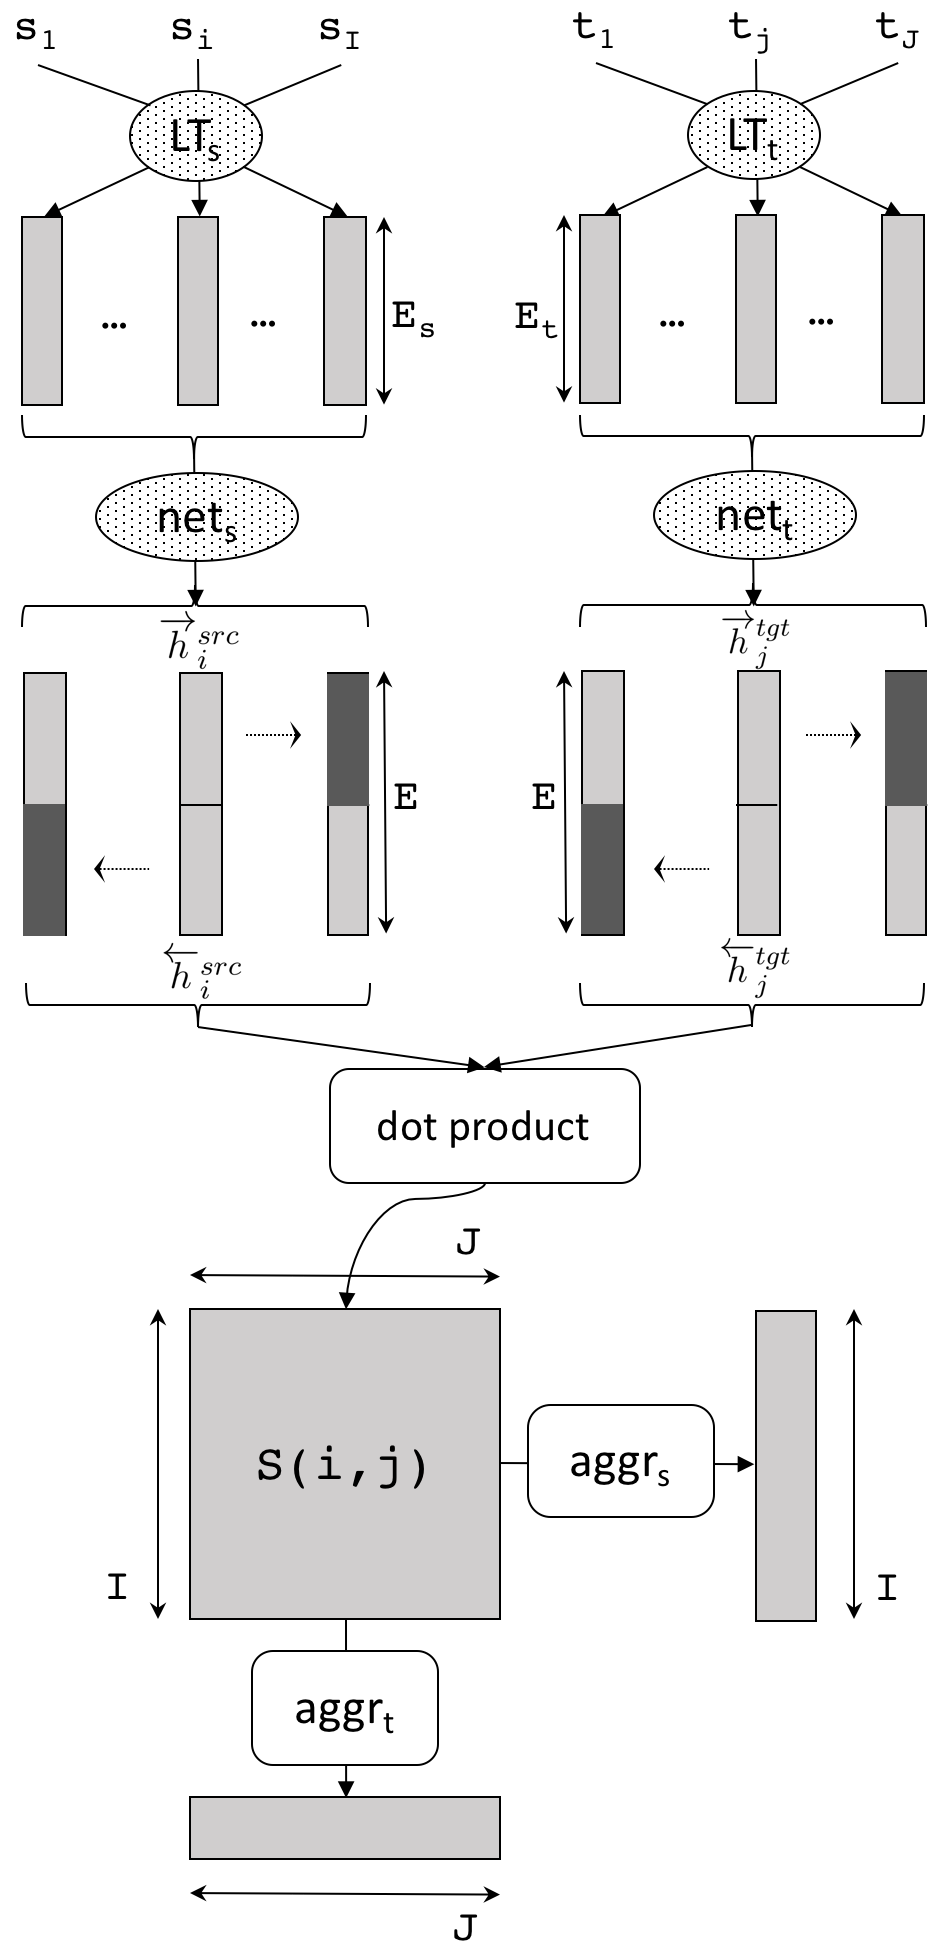
\includegraphics[width=1.0\linewidth]{network}
    \caption{Illustration of the model. The network is composed of source and target word embedding lookup tables ($LT_s$ and $LT_t$) and two identical subnetworks ($net_s$ and $net_t$) that compute in context representations of source ($s_i$) and target words ($t_j$).} 
    \label{network}
\end{figure}


At this point a measure of similarity between sentences can be obtained by cosine similarity: 
\begin{equation}
    sim(h_{src}, h_{tgt}) = \frac{h_{src} \cdotp h_{tgt}}{||h_{src}|| * ||h_{tgt}||}
    \label{cosine}
\end{equation}
\noindent where two vectors (embeddings) with the same orientation have a cosine similarity of $1$, while two vectors with opposed orientation have a similarity of $-1$, independent of their magnitude.

%The similarity function outputs the level of semantic similarity between source and target sentences.

%Figure~\ref{net_lstm} illustrates the first component of our network. In order to optimise our model we follow the functions depicted in Figure~\ref{net_align}.

Similar to ~\cite{W16-2207} our model extracts context information from source and target sentences and then computes simple dot-products to estimate word alignments. 
The objective function is computed at the level of words. 
To enable unsupervised training, we use an aggregation operation that summarizes the alignment scores for a given target word. 
A soft-margin objective increases scores for true target words while decreasing scores for target words that are not present.
The aggregation function combines the scores of all source (or target) words for a particular target (or source) word and promotes source words which are likely to be aligned with a given target word according to the knowledge the model has learned so far.
Alignment scores $S(i,j)$ are given by the dot-product $S(i,j) = h_i^{src} \cdotp h_j^{tgt}$, while aggregation functions are defined as:

\begin{equation}
\begin{split}
    aggr_s(i,S) = \frac{1}{r} \ log \left( \displaystyle \sum_{j=1}^{J} e^{r * S(i,j)}\right) \\
    aggr_t(j,S) = \frac{1}{r} \ log \left( \displaystyle \sum_{i=1}^{I} e^{r * S(i,j)}\right)
\end{split}
\label{aggregation}
\end{equation}

%Hence, rather than sentence similarity our model optimises word alignments.
The loss function is defined as:

%\vspace{-8mm}
\begin{equation}
\begin{split}
\mathcal{L}(src,tgt) = & \\
    \sum_{i=1}^I log&\left(1+e^{aggr_{s}(i,S) * \mathcal{Y}_i^{src}}\right) +\\
 + \sum_{j=1}^J log&\left(1+e^{aggr_{t}(j,S) * \mathcal{Y}_j^{tgt}}\right)
\end{split}
\label{loss_wemb}
\end{equation}
\noindent where $\mathcal{Y}_i^{src}$ and $\mathcal{Y}_j^{tgt}$ are vectors with reference labels containing $-1$ when the word is present in the translated sentence, and $+1$ for divergent (unpaired) words. 

%\begin{figure}[h]
%\center
%    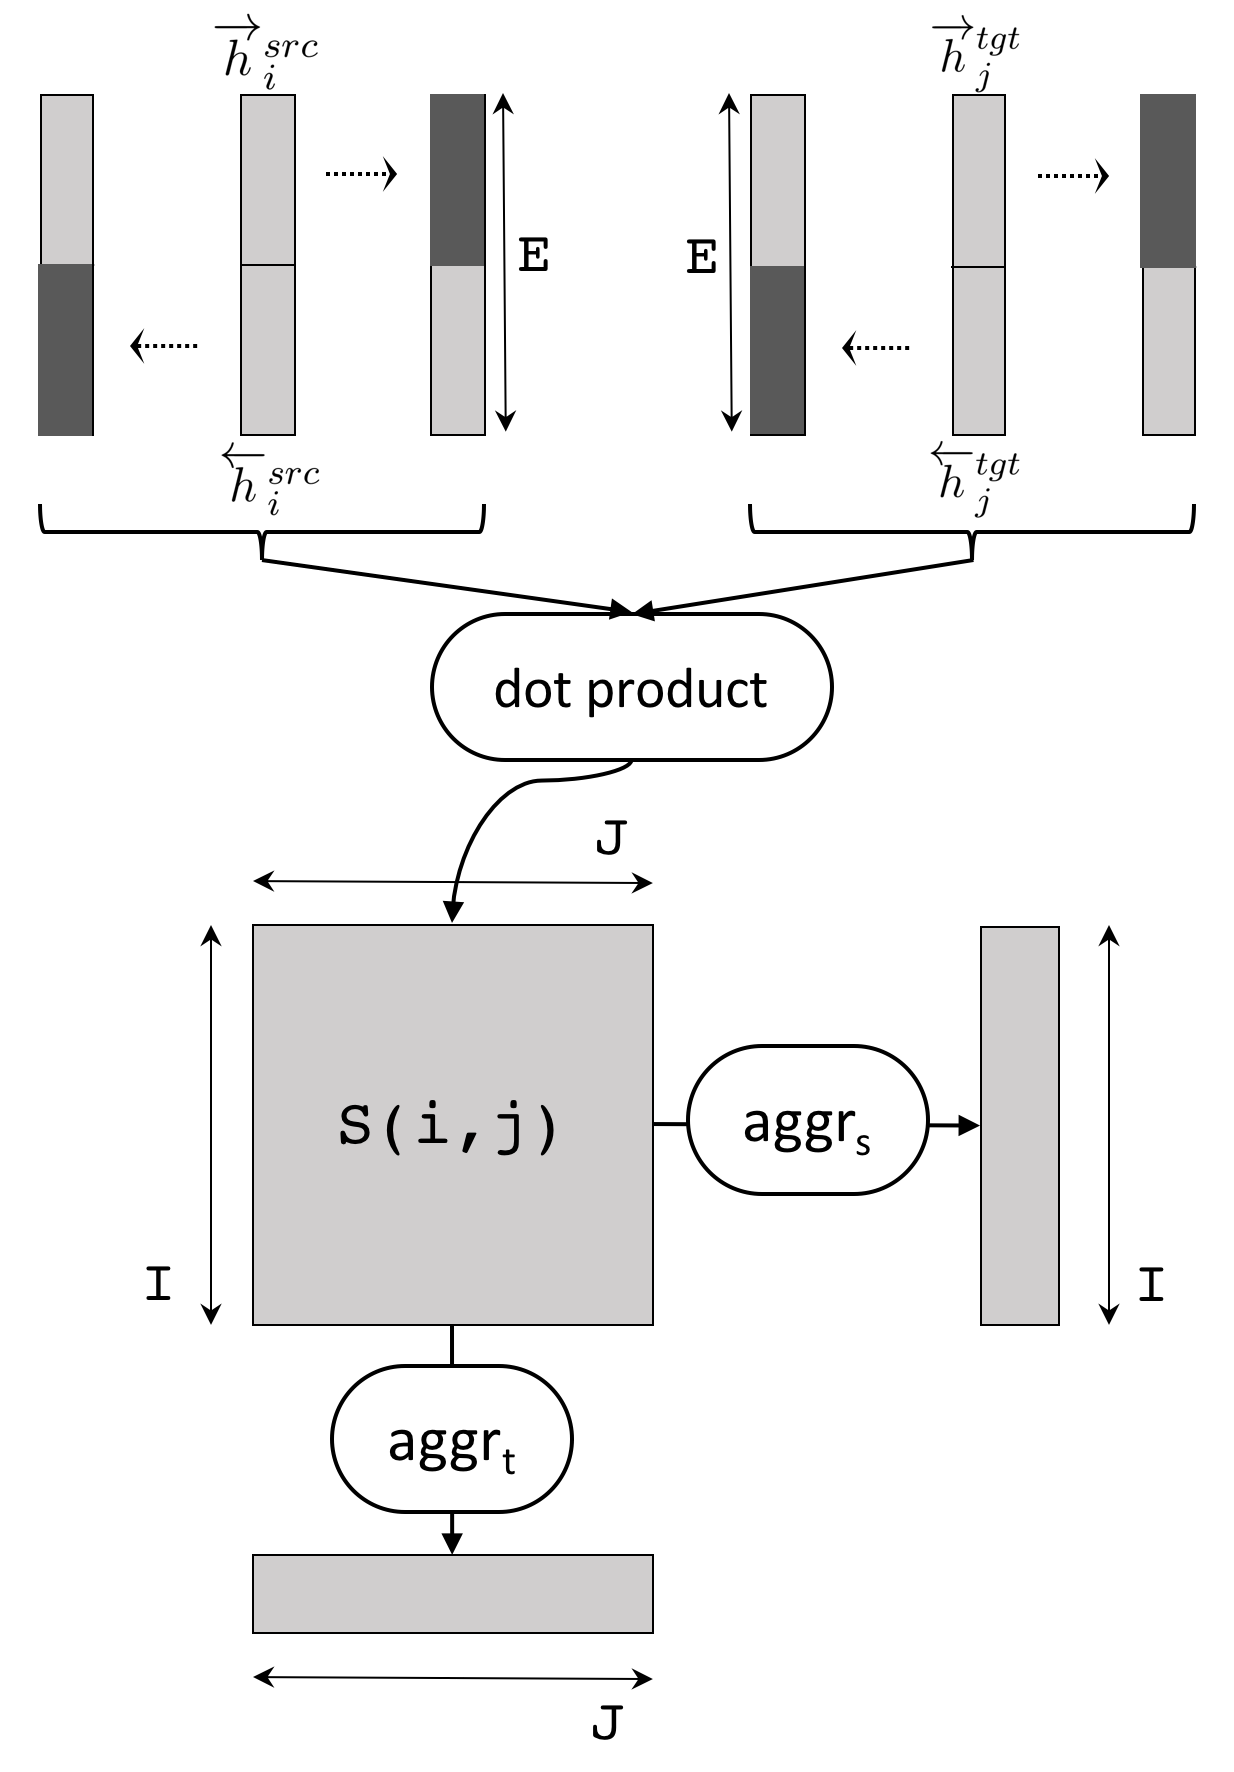
\includegraphics[width=0.9\linewidth]{net_align}
%    \caption{Illustration of the model.}
%    \label{net_align}
%\end{figure}

%\vspace{-8mm}

%For comparison purposes we also implemented the model introduced in \cite{W17-2509}. The network employs the same initial Bi-LSTM layers outlined in Figure~\ref{network} which encode source and target sentences into $h_{src}$ and $h_{tgt}$ vectors. The remaining of the network is illustrated by Figure~\ref{net_sentence}, where sentence pair matching information is captured by using their element-wise product and absolute element-wise difference. Sentence similarities are finally estimated by feeding the matching vectors into a fully connected layer.

%\begin{equation}
%\begin{split}
%h^{(1)} =  &\ \ h_{src} * h_{tgt} \\
%h^{(2)} =  &\ \ |h_{src} - h_{tgt}| \\
%h^{(3)} = &\ \ tanh(W[h^{(1)};h^{(2)}] + b^{(3)}) \\
%h_{sim} = &\ \ Wh^{(3)} + b^{sim}
%\end{split}
%\end{equation}

%This approach is different from our model since it uses a single end-to-end model to estimate the conditional probability distribution that two sentences are parallel. 

%\begin{figure}[h]
%\center
%    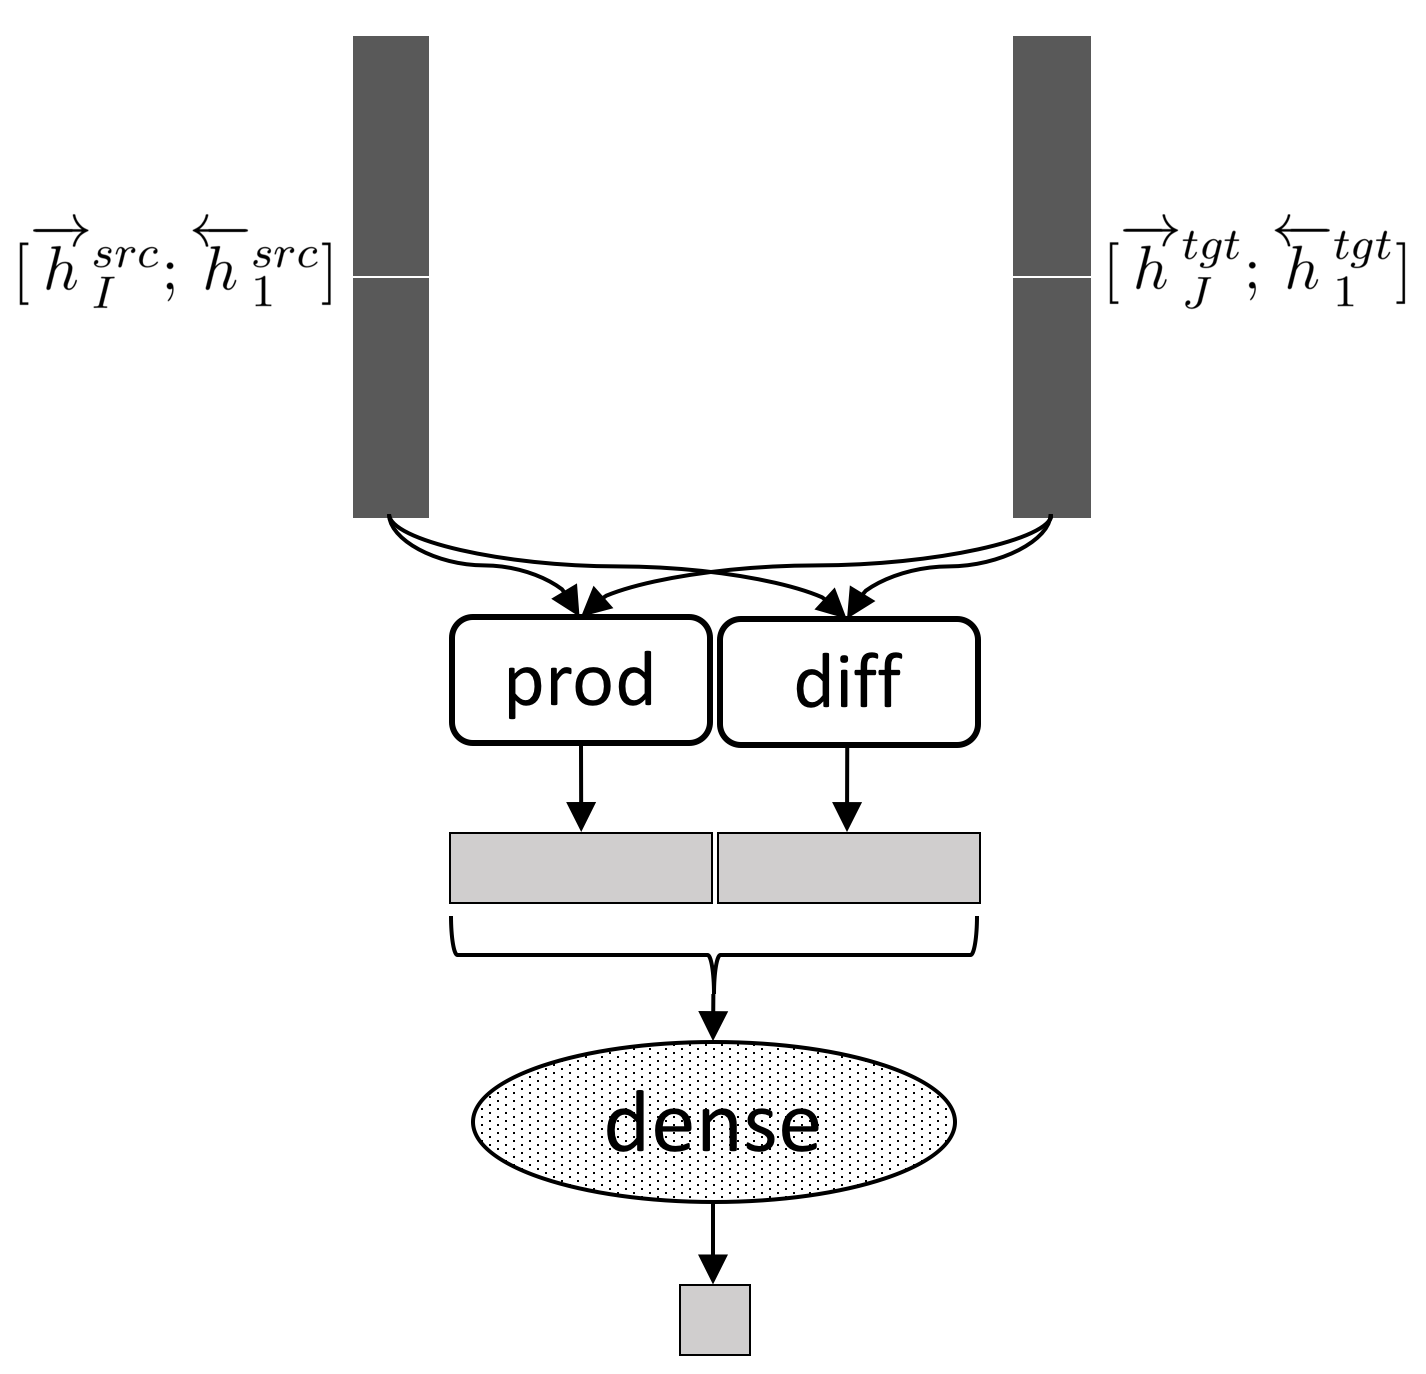
\includegraphics[width=0.8\linewidth]{net_sentence}
%    \caption{Illustration of the model presented in~\cite{W17-2509}. Sentence embeddings (vectors in dark grey) are computed by the same Bi-LSTM layers shown in Figure~\ref{network}.} %The network is composed of source and target word embedding lookup tables ($LT_s$ and $LT_t$) and two identical subnetworks ($net_s$ and $net_t$) that compute in context representations of source ($s_i$) and target words ($t_j$). The similarity function outputs the level of semantic similarity between source and target sentences.}
%    \label{net_sentence}
%\end{figure}

%For this second network the loss function is defined as: 
%\vspace{-5mm}
%\begin{equation}
%\mathcal{L}(src,tgt) = log(1+e^{h_{sim} * \mathcal{Y})}) % where $sign(src,tgt) =1
%\label{loss_semb}
%\end{equation}
%\noindent where $\mathcal{Y}$ is the reference label containing $-1$ when the given sentence pair is non-divergent (parallel) and $+1$ for divergent (unpair) examples. 

%Note that different from the network described in the original work, our implementation does not estimates a probability distribution but FINISH.

%For each source(target) word, we consider the aggregated matching score over the target(source) sentence:
%$$s_{aggr}(i,tgt) = Aggr_{j=1}^{J} s(i,j)$$
%$$s_{aggr}(src,j) = Aggr_{i=1}^{I} s(i,j)$$

%Where $Aggr$ is LSE aggregation operator used in~\cite{W16-2207}. Given the sign of each word noted $sign(w)$, that indicates whether the word $w$ is matched to the other side (by convention, $1$ indicates non-matching, $-1$ indicates matching), the loss function is defined as follows:


%In the second option, we directly optimize the score of similarity between two sentences by defining the loss function as follows:

%$$L(src,tgt) = log(1+e^{h_{src} . h_{tgt} * sign(src,tgt)})$$ where $sign(src,tgt) =1 $ if two sentences are not parallel and $sign(src,tgt) =-1 $ otherwise.

\subsection{Training with Negative Examples}
\label{training}

Training is performed by minimising Equation~\ref{loss_wemb}, for which examples with annotations for source $\mathcal{Y}_i^{src}$ and target $\mathcal{Y}_j^{tgt}$ words are needed.
Different kind of examples are used to train our network:
\begin{itemize}

\item As positive examples we use paired sentences of the parallel corpus. In this case, all words in both sentences are labelled as parallel, $\mathcal{Y}_i^{src}=-1$ and $\mathcal{Y}_j^{tgt}=-1$. 

\item As negative examples we use random unpaired sentences. In this case, all words are labelled as divergent, $\mathcal{Y}_i^{src}=+1$ and $\mathcal{Y}_j^{tgt}=+1$. 
Since negative examples may be very easy to classify and we want our network to detect less obvious divergencies, we further create negative examples following the next two methods:

\item We replace random sequences of words on either side of the sentence pair by a sequence of words with the same part-of-speeches. 
The rationale behind this method is to keep the new sentences as grammatical as possible. 
Otherwise, to predict divergence the network can learn to detect non-grammatical sentences.
Words that are not replaced are considered parallel ($-1$) while those replaced are assigned the divergent label ($+1$). 
Words aligned to some replaced words are also assigned the divergent label ($+1$). For instance, given the original sentence pair:

\begin{table}[h]
\center
\begin{tabular}{ll}
src: & { \small \texttt{What do you feel ?}} \\
tgt: & { \small \texttt{Que ressentez-vous ?}} \\
\end{tabular}
\end{table}

We may replace '\texttt{you feel}', with part-of-speech tags '\texttt{PRP VB}', by another sequence with same tags (i.e. '\texttt{we want}'):

\begin{table}[h]
\center
\begin{tabular}{ll}
src: & { \small \texttt{What do {\bf we \ want} ?}} \\
$\mathcal{Y}^{src}$: & { \small \texttt{-1 \ \  -1 {\bf +1\ \ +1} \ \  -1}} \\
tgt: & { \small \texttt{Que {\bf ressentez-vous} ?}} \\
$\mathcal{Y}^{tgt}$: & { \small \texttt{-1\ \ {\bf +1}\ \ \ \ \ \ \ \ \ -1}} \\
\end{tabular}
\end{table}

Divergent words are shown in bold. 
Note that the new sentences are not assured to be grammatical after replacing sequences with the same part-of-speech.
We use word alignments to identify as divergent the sequence '\texttt{ressentez-vous}' since it is aligned to '\texttt{you feel}' in the original sentence pair.

\item Finally, motivated by sentence segmentation errors observed in many corpora, we also build negative examples by inserting a second sentence at the beginning (or end) of the source (or target) sentence pair. 
Words in the original sentence pair are assigned the parallel label ($-1$) while the new words inserted are considered divergent ($+1$).
Given the original sentence pair previously shown, we may want to build the next negative example by inserting the sentence '\texttt{Not .}' at the end of the original source sentence:

\begin{table}[h]
\center
\begin{tabular}{ll}
src: & { \small \texttt{What do you want ? {\bf Not \ .}}} \\
$\mathcal{Y}^{src}$: & { \small \texttt{-1 \ \  -1 -1 \ -1  \ \ -1 {\bf +1\ \ \  +1}}} \\
tgt: & { \small \texttt{Que ressentez-vous ?}} \\
$\mathcal{Y}^{tgt}$: & { \small \texttt{-1\ \ -1\ \ \ \ \ \ \ \ \ \ \ \ \ -1}} \\
\end{tabular}
\end{table}

\end{itemize}

In order to avoid that negative examples are easily predicted just by looking at the difference in length of training sentences we constraint all negative examples to have a difference in length not exceeding $2.0$. Very short sentences, of up to $4$ words, are accepted if the length ratio does not exceeds $3.0$.
Note that the network can be trained with any combination of examples ({\texttt P}aired, {\texttt U}npaired, {\texttt R}eplace and {\texttt I}nsert).
In all cases, the same number of examples is used for each type.


\subsection{Fixing Translation Divergencies}
\label{correction}

We observed in our training corpora that many divergent sentences follow a common pattern, consisting of adding some extra leading/trailing words.
As in the first and second examples of table~\ref{tab:examples}.
Accordingly, we implemented a simple algorithm that discards sequences of leading/trailing words on both sides of the source and/or target sentences. 
Hence considering as parallel $s_u^v$ and $t_x^y$. 
To find the optimal source ($u, v$) and target ($x, y$) indices that enclose the parallel segments within the original sentence, we implement:
\begin{equation*}
\underset{u, v, x, y}{\arg\max} \Big \{      \underset{u \le I \le v}{\sum} \underset{x \le j \le y}{\max} \{ S(i,j) \}    \Big \}
\end{equation*}

The $\mathcal{N}$-best sequences following the previous function ($s_u^v$, $t_x^y$) are considered as valid corrections, but only the highest ranked according to its similarity score is used as replacement for the original $(s_1^I, t_1^J)$.
Short sentences are not considered. This is, $v - u > \tau$ and $y - x > \tau $. 
Figure~\ref{matrix} (left) shows an example of an alignment matrix $S(i,j)$ for a given sentence pair. 
An acceptable correction is: 

\begin{table}[h]
\center
\begin{tabular}{c}
	\textit{Que ressentez-vous ? \ \ $\Leftrightarrow$\ \ \ What do you feel ?} \\
\end{tabular}
\end{table}


\noindent Hence, with optimal indices being: $u=1$, $v=5$, $x=1$ and $y=3$.

\section{Experiments}
\label{experiments}

In this section we report on the experiments conducted to evaluate the proposed network. We begin with details of the corpora employed.

\subsection{Corpora}
\label{corpora}

Different corpora are used in this work to evaluate our similarity classifier.
We filter out divergencies found in the English-French OpenSubtitles corpus~\cite{LisonTiedemann2016}, which consists of a collection of movie and TV subtitles, aligned at the sentence level after a number of automatic preprocessing steps. 
The corpus presents many potential divergencies as outlined in Table~\ref{tab:examples}. 
To evaluate performance we used the En-Fr Microsoft Spoken Language Translation task, created from actual conversations over Skype~\cite{mslt-corpus-iwslt-2016-release}. 
%We also tested on a second domain, using the publicly available newstest-2013 En-Fr test set, corresponding to news stories selected from online sources~\cite{WMT:2013}.

In order to better assess the quality of our classifier when facing different types of word divergences we collected from the original OpenSubtitles corpus $500$ sentences containing different types of examples:
\begin{itemize}
\item $200$ paired sentences,
\item $100$ unpaired sentences,
\item $100$ sentences with replace examples and
%\item $100$ sentences with replace examples; 
\item $100$ sentences with insert examples.
\end{itemize}

Details of each type of example are given in Section~\ref{training}.
Sentence pairs have divergence annotations at the level of words.

We also use the Paracrawl corpus, which consists of a very noisy $1$ billion word (English token count) German-English corpus crawled from the web as part of the Paracrawl project\footnote{http://paracrawl.eu/}.
Performance is evaluated on the publicly available newstest-2017 En-De test set, corresponding to news stories selected from online sources~\cite{W17-4717}.

%To evaluate the ability of our sentence embeddings to identify parallel sentences in comparable corpora we followed the data conditions made available for the BUCC shared task~\cite{ZWEIGENBAUM18.12}. 
%For training we used the French-English European Parliament corpus from WMT15\footnote{http://www.statmt.org/wmt15/translation-task.html}.
%For testing we used the test set made available by the task organisers, consisting of about $300,000$ monolingual sentences per language, French and English, that contains near $10,000$ parallel sentences.
%Test data come from Wikipedia\footnote{http://ftp.acc.umu.se/mirror/wikimedia.org/dumps} and News Commentary\footnote{http://www.casmacat.eu/corpus/news-commentary.html}.

\subsection{Training}

All data is preprocessed with \texttt{OpenNMT}\footnote{http://opennmt.net}, performing minimal tokenisation, basically splitting-off punctuation.

\subsubsection{Neural Similarity Classifier}
\label{divergence}

After tokenisation, the $50,000$ most frequent words of each language are used as vocabulary.
Each out-of-vocabulary word is mapped to a special UNK token.
Our similarity classifier is described in Section~\ref{sec:similarity}. 
Word embeddings ($LT_s$ and $LT_t$) are initialised using \texttt{fastText}\footnote{https://github.com/facebookresearch/fastText}, further aligned by means of \texttt{MUSE}\footnote{https://github.com/facebookresearch/MUSE} following the unsupervised method detailed in~\cite{lample2018word}. 
Size of embeddings is $E_s=E_t=256$ cells. 
Both Bi-LSTM use 256-dimensional hidden representations ($E=512$). 
We use $r=1.0$. 
Optimization of the parameters is done using the stochastic gradient descent method along with gradient clipping (rescaling gradients whose norm exceeds a threshold) to avoid the exploding gradients problem~\cite{Pascanu:2013:DTR:3042817.3043083}. 
For each epoch we randomly select $1$ million sentence pairs that we place in batches of $32$ examples.  
Negative examples are created following the strategies detailed in~\ref{training}.
Word alignments and English part-of-speeches used to build negative examples were performed by \texttt{fast\_align}\footnote{https://github.com/clab/fast\_align} and \texttt{FreeLing}\footnote{https://github.com/TALP-UPC/FreeLing.git} respectively.
We run $10$ epochs and start decaying at each epoch by $0.8$ when score on validation set increases. 
Divergence is always computed following equation~\ref{cosine}. 
For divergence correction, we use $\mathcal{N}=20$ and $\tau=3$.

\subsubsection{Neural MT}
\label{translation}

In addition to the basic tokenisation detailed in Section~\ref{divergence} we perform Byte-Pair Encoding~\cite{Sennrich2016} with $30000$ merge operations learned joined from both language sides.
Neural MT systems are based on the open-source project  \texttt{OpenNMT}. 
We use a Transformer model with same configuration than in paper~\cite{vaswani2017attention}, i.e, both encoder and decoder have $6$ layers; Multi-head attention is performed over $8$ heads. 
Hidden layer�s size is $512$. 
The inner layer of feed forward network is of size $2048$. 
Word embeddings have $512$ cells. We set the dropout probability to $0.1$. 
Batch size is set to $3072$.
%The maximum length of both source and target sentences is set to $80$ and we limit the vocabulary size to $50,000$ words for both source and target languages. 
The optimiser is Lazy Adam with $\beta_1 = 0.9$, $\beta_2 = 0.98$, $\epsilon = 10^{-9}$, $warmup\_steps = 4000$. We stop training after $30$ epochs.


%In addition to the basic tokenisation we perform Byte-Pair Encoding~\cite{Sennrich2016} with $30,000$ merge operations learned from both English and French data.
%We build our NMT systems based on the open-source project \texttt{OpenNMT}. We use a bidirectional RNN encoder with $4$ LSTM layers with each containing $1,000$ cells. Word embeddings have a size of $300$ cells. We set the dropout probability to $0.3$. Batch size is set to $64$. The maximum length of both source and target sentences is set to $80$. % and we limit the vocabulary size to $50K$ words for both source and target languages.
%The default optimiser is SGD with the starting learning rate of $1.0$. We start to decay the learning rate from epoch $10$ or when we detect increasing perplexity as compared to the previous epoch on a validation set. We stop training after $20$ epochs.


\section{Results}
\label{sec:results}

We evaluate first the ability of our similarity classifier to predict different types of divergencies at the level of words. 
We use the test set manually annotated for that purpose and train our model on the OpenSubtitles corpus.
A word is considered divergent when associated to a negative aggregation score (see Equation~\ref{aggregation}).
Table~\ref{results_puri} shows accuracies obtained by our model when trained over different combinations of negative examples.% on the task of predicting wether words are divergent. 
%We consider as divergent those words for which the similarity score predicted by our model, Equation~\ref{cosine}, is negative.

\begin{table}[h]
\small
\center
\begin{tabular}{crccccc}
\hline
\multicolumn{2}{l}{\bf Accuracy} & \multicolumn{5}{c}{Test examples} \\
 &  & \texttt{P} & \texttt{U} & \texttt{R} & \texttt{I} & \texttt{PURI} \\
 \hline
\parbox[t]{0mm}{\multirow{7}{*}{\rotatebox[origin=c]{90}{Train examples}}} &  \texttt{PU}     & \bf 0.996 & \bf 0.994 & 0.671 & 0.673 & 0.874 \\
 &  \texttt{PR}     & \bf 0.995 &      0.033 & \bf 0.951 &      0.689 & 0.746 \\
 &  \texttt{PI}       & \bf 0.998 &      0.071 &      0.697 & \bf 0.725 & 0.705 \\
 &  \texttt{PUR}  & \bf 0.994 & \bf 0.989 & \bf 0.919 &      0.710 & 0.932 \\
 &  \texttt{PUI}    & \bf 0.995 & \bf 0.996 &      0.662 & \bf 0.769 & 0.887 \\
 &  \texttt{PRI}    & \bf 0.991 &      0.161 & \bf 0.924 & \bf 0.719 & 0.768 \\
 &  \texttt{PURI} & \bf 0.995 & \bf 0.980 & \bf 0.916 & \bf 0.788 & \bf 0.942 \\
\hline
\end{tabular}
\caption{Word divergence accuracies according to different type of examples used in train/test. P, U, R and I stand respectively for pair, unpair, replace and insert.}
\label{results_puri}
\end{table}

As it can be seen, non-divergent words in parallel sentences (column \texttt{P}) are easy to identify. 
In all cases the accuracy reaches $100\%$. 
Divergent words in unpaired sentences (column \texttt{U}) are also easy to identify as far as the model has seen these types of examples in training. 
However, the accuracy drops dramatically when the model is not trained with unpaired sentences (rows  \texttt{PR}, \texttt{PI} and \texttt{PRI}).
Regarding columns \texttt{R} and \texttt{I}, accuracies are lower since these sentences contain a mix of divergent and non-divergent words. 
%Hence, word divergence is more difficult to predict. 
Again, models that were trained with the corresponding examples (\texttt{R} and \texttt{I}) obtain the highest accuracies (outlined in bold letters).
Column \texttt{PURI} shows accuracy results over the entire test set. This is, mixing all type of examples. 
As expected, the best accuracy is also obtained by the system trained on all type of  examples. 

%The test set was annotated after looking at the entire train set and looking for these type of examples. 
%Existance and distribution of types of 

\begin{figure}[h]
\centering
    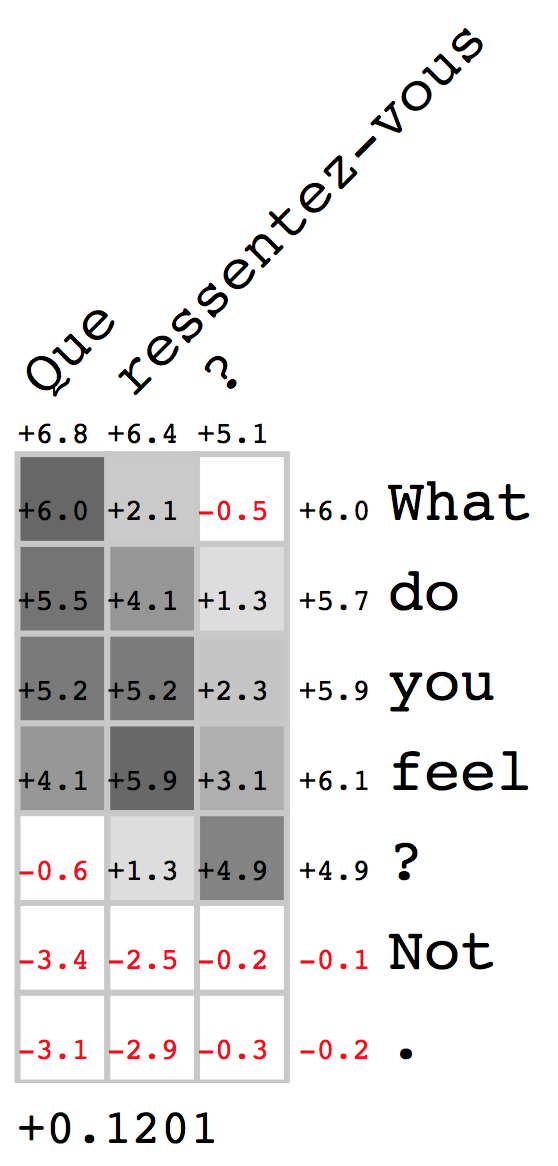
\includegraphics[width=0.4\linewidth]{feel}    
    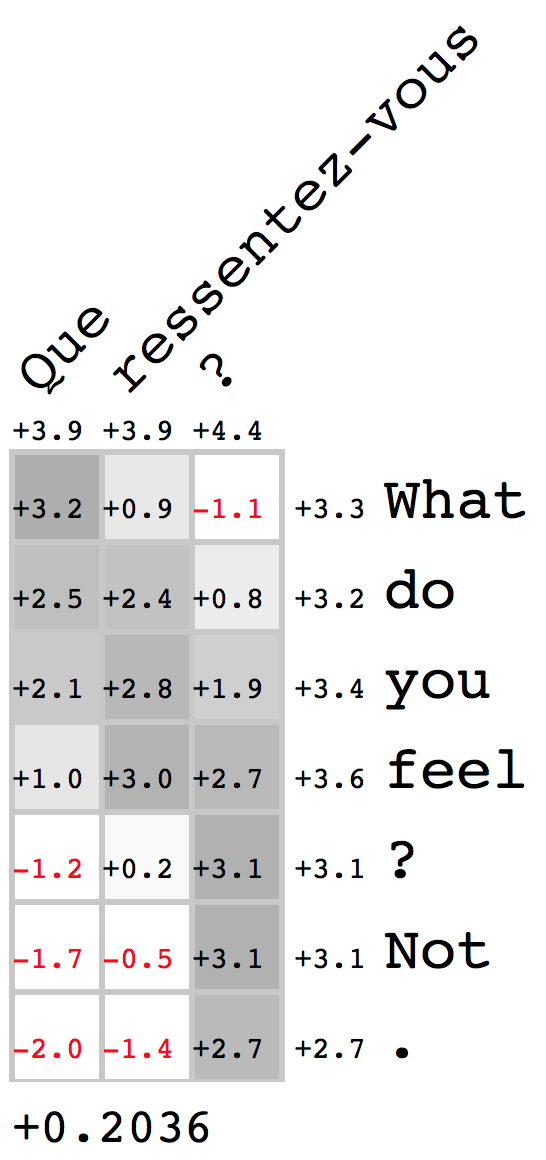
\includegraphics[width=0.4\linewidth]{feel_pu}    
\caption{Sentence pair with similarity scores produced by our model when trained over \texttt{PU} examples (right) and over \texttt{PURI} examples (left). Aggregation scores (Equation~\ref{aggregation}) are shown next to words. Matrices contain alignment scores. Sentence similarities (Equation~\ref{cosine})  shown below matrices.}
\label{matrix}
\end{figure}

Figure~\ref{matrix} illustrates the output of our network when trained using \texttt{PU} examples (right) and \texttt{PURI} examples (left).  
The former (right) fails to predict some word divergences, most likely because in training it never saw sentences mixing divergent and non-divergent words in the same example. 
Furthermore, the network trained over \texttt{PURI} examples (left) correctly assigns a lower similarity score to the sentence pair as both sentences do not convey the exact same meaning.

Next, we evaluate the ability of our neural similarity classifier to detect divergent sentence pairs. 
Since we lack of a gold standard test set to directly evaluate sentence similarity, 
we measure the accuracy of neural MT systems trained over the original corpus and after filtering divergent sentences. 
Notice that some divergent sentences may not be completely useless to train a neural MT system. 
Consider for instance the example of Figure~\ref{matrix}. 
Despite not conveying the exact same meaning it still contains useful information to train a neural MT engine. 
It is not the case of the example in the third row of Table~\ref{tab:examples}.

Table~\ref{results_wemb} shows BLEU~\cite{P02-1040} scores of the same neural MT network when trained over different samples of the OpenSubtitles corpus.
Samples result from filtering sentences of the original corpus using different similarity thresholds.

\begin{table}[h]
\small
\center
\begin{tabular}{lcc}
\hline
\bf $sim(h_{src},h_{tgt})$ & \bf Size (M) & \bf Test (BLEU)\\%& \bf NEWS \\
\hline
$(-\infty,+\infty)$   & 27.2 & 42.18 \\ %& 26.60  \\
$[0.000,+\infty)$   & 24.0 & 42.68 \\ %& 26.87  \\
$[0.003,+\infty)$   & 21.5 & 42.56 \\ %&  \\
$[0.076,+\infty)$   & 18.0 & \bf 43.19 \\ %& 26.38 \\
$[0.100,+\infty)$   & 15.5 & \\%&  \\
\hline
\end{tabular}
\caption{BLEU scores obtained by a neural MT network when trained over the OpenSubtitles corpus filtered using different similarity thresholds.}
\label{results_wemb}
\end{table}

As it can be seen, the best performing training sample is obtained when using sentence pairs with similarity score in the range $[0.076, +\infty)$. 
This is, training with the most similar $18$ million sentences of the original data set. 
Note that despite assigned a positive similarity score, sentence pairs in the range $[0, 0.076]$ (almost $10$ million sentences) does not seem to contribute when training a neural MT network. 
On the contrary, when added as training data the MT accuracy is reduced.

Table~\ref{results} shows BLEU results for our neural MT engine trained over different data configurations:
The entire\footnote{The original Paracrawl corpus contains more than $100$ million sentences. We reduced its size to $22.2$ millions using standard filtering techniques.} data sets (\texttt{all}) of both corpora; 
Most similar pairs after as predicted by our network (\texttt{sim}); 
Finally, we apply the correction algorithm detailed in Section~\ref{correction} (\texttt{sim+fix}).
Columns Ref and Fix indicate the number of original and corrected sentences (in millions) considered to train the neural MT system.

\begin{table}[h!]
\small
\center
\begin{tabular}{lccl}
\hline
\bf Data & \bf Ref (M) & \bf Fix (M) & \bf Test (BLEU) \\ %MSLT & \bf NEWS \\
\hline
\multicolumn{3}{c}{\scriptsize{OpenSubtitles English-French}} \\
\texttt{all}                   & 27.2 & - & 42.18 \\
%\texttt{semb}             & 18.0 & - & \\
\texttt{sim}            & 15.5 & - & 43.12  ($+0.94$)\\
%\texttt{sim}           & 21.5 & - & 42.56 \\
\texttt{sim}           & 18.0 & - & 43.19  ($+1.01$)\\
\texttt{sim+fix}     & 15.5 & 2.5 & \bf 44.19 ($+2.01$)\\
%\texttt{sim+fix}   & 15.5 & 5.0 & \\
\hline
\multicolumn{3}{c}{\scriptsize{Paracrawl English-German}} \\
%\texttt{all}                  & 100.0 & 12.56 \\ 
\texttt{all}                  & 22.2 & - & 19.27 \\ 
%\texttt{semb}            & 15.0 & - & \\
\texttt{sim}           & 15.0 & - & 21.52 ($+2.25$)\\
\texttt{sim}           & 17.5 & - & 21.97 ($+2.70$)\\
\texttt{sim+fix}   & 15.0 & 2.5 & \bf 22.42 ($+3.15$) \\
\hline
\end{tabular}
\caption{BLEU scores obtained by neural MT using different subsets of the OpenSubtitles and Paracrawl corpora.}
\label{results}
\end{table}

Results obtained after filtering sentence pairs by our network, \texttt{sim}, clearly outperform the baseline \texttt{all} by $+0.94$ and $+2.25$ BLEU respectively.

Regarding OpenSubtitles, when fixing $2.5$ million sentences ($4^{th}$ row) the accuracy is further boosted to $+2.01$, while the same sentence pairs does not show any improvement when added in their original form ($3^{rd}$ row).
%results are further improved $+2.01$ when fixing $2.5$ million sentences ($4^{th}$ row). 
%The same $2.5$ million sentences did not show any improvement when added in their original form 

Similar results are obtained over the Paracrawl corpus. Results after fixing $2.5$ million sentences ($4^{th} row$) outperform those obtained by the same same sentence pairs when used by the neural MT system in their original form ($3^{rd} row$).

\section{Conclusions}
\label{conclusions}

We presented an unsupervised method based on deep neural networks for detecting translation divergences in parallel sentence pairs. 
Our model optimises word alignments. Hence, allowing for fine grained divergence prediction at the level of words. 
Misaligned/divergent words can then be filtered out allowing for reusing some divergent sentences. 
We evaluated our model on two neural machine translation tasks, showing significant improvements when compared to training over the entire data set. 
The method can be used on any parallel corpus without any manual annotation.

\section{Further Work}
\label{further}

%We plan to further evaluate divergence classification under different data noise levels. %and on additional language pairs. 
%as well as to measure the impact of using less noisy data when learning the similarity model
%We also would like to evaluate the impact of using less noisy (already filtered) data to learn the similarity model. 
%We would also like to use our model to predict other types of divergences 
We plan to use our model to predict sentence embeddings over comparable corpora, allowing to collect parallel pairs through vector similarity measures.
%We also plan to further evaluate the correction algorithm.
In addition, we would like to measure the performance of our model after applying subword tokenisation,
%when working with a reduced vocabulary set, as a result of applying any subword tokenisation,
as well as using multiple LSTM layers, which is well known to capture hierarchical structure in the context of MT.


%\section*{Acknowledgements}
%We are grateful to Jo\"el Legrand for his fruitful comments when building the neural divergence classifier.

\bibliography{biblio}
\bibliographystyle{acl_natbib_nourl}

\end{document}
